\chapter{Detecção de Intrusão em um Cenário Real} \label{ch:cenário-real}
 %- Em cada capitulo adicionar um texto introdutório

Este capítulo esta organizado da seguinte forma: A próxima seção apresenta o cenário de testes, descrevendo características gerais da rede selecionada para os teste. Na seção \ref{sec:infraestrutura} será abordado a infraestrutura usada para os testes, ferramentas utilizadas e as configurações feitas. Na seção \ref{sec:testes} será descrito os testes realizados com suas respectivas justificativas. Na seção \ref{sec:resultados} será apresentado os resultados esperados e obtidos, problemas encontrados e a comparação das ferramentas e por último, na seção \ref{sec:conclusão}, uma breve conclusão.

\section{Metodologia dos Testes}

Nessa seção será descrito o cenário utilizado para a realização dos testes. Na \autoref{sec:cenário}, aborta a rede onde os sensores foram instalados e algumas de suas estatísticas de uso. A \autoref{sec:infraestrutura} descreve a infraestrutura montada para realização dos testes, os equipamentos utilizados e as ferramentas adicionais. Na \autoref{sec:testes}, será descrito os testes realizados. Na \autoref{sec:resultados} abordará os resultados esperados e obtidos com os testes. Por último, na \autoref{sec:conclusão} a conclusão.

% (Adicionar o escopo dos testes): descrever o ambientes,
\subsection{Cenário de Testes} \label{sec:cenário}
%Descrever o cenário. Ex: Uma rede com XXX usuários; Os usuários utilizam
%diferentes ferramentas,...
%Adicionar gráficos de utilização da rede

\subsection{Infraestrutura Definida para Testes} \label{sec:infraestrutura}
%Descrever o que foi utilizado:
%Ex: Equipamentos - Servidores, ....
%    Configuração
%    Ferramentas - Snort (referenciar capítulo), ...

No ambiente de teste foi usado uma máquina Dell com 134 Megabytes (MB) de memória RAM e 40 núcleos. Usou-se XenServer \cite{xenserver} versão 7, sistema operacional (SO) \textit{opensource} da Citrix voltado para virtualização. Foram testados outros SOs porém somente o XenServer possuía, na época da instalação do ambiente, \textit{firmware} da placa de rede do \textit{host} compatível e que funcionava com instabilidade. 
 
Outro fator que pesou na escolha do SO foi a experiência com a plataforma e por existir uma interface para gerencia chamada XenCenter que roda no Windows. Uma alternativa \textit{opensource} desse software é o OpenXenManager que funciona nos sistemas Unix \cite{openxenmanager}.

No primeiro momento, foi instalado uma máquina virtual com o sistema operacional Debian 9.3 \textit{codename} Wheezy \cite{debianwheezy}, uma distribuição linux com uma proposta de ser totalmente livre, usada como base para instalação de outras máquinas utilizando o recurso de \textit{snapshot}, uma cópia de uma máquina virtual rodando em um certo momento, do XenServer. O uso desse recurso foi necessário para criar um ambiente igual para os IDSs.

Foi alocado 8 MB memória RAM, 4 processadores e 100 Gigabytes(GB) de espaço em disco para o \textit{snapshot}. Esses valores foram definidos com base em um estudo \cite{mikelococo} que considerava vários fatores, como largura da rede, localização do IDS e versão, tipo do capturador de tráfego e tamanho da base de assinaturas para dimensionar os recursos de memória e processamento, aplicado especificamente ao Snort. A mesma regra foi aplicada ao Suricata.

Para o \textit{host} conseguir pegar o pacotes destinados a rede escolhida para ser monitorada foi necessário uma configuração de espelhamento no roteador B (Figura \ref{fig:infra-ambiente}) que consiste na copia dos pacotes que saem pela porta dessa rede no roteador para a porta conectada no \textit{host} que possui uma largura de banda de 10 Gigabits. A interface de rede do \textit{host} precisou ser configurada no modo \textit{promisc}.

Posteriormente criou-se quatro máquinas virtuais, duas usadas para instalação dos IDSs (Suricata e Snort) e a terceira para instalação das ferramentas usadas para simular ataques a rede. Optou-se pela instalação do sistema Kali Linux \cite{kalilinux} para geração de ataques pois nele existe várias ferramentas nativas para testes de penetração e auditoria de segurança (Metasploit \autoref{sec:metasploit}, NMAP \autoref{sec:nmap} e OpenVAS \autoref{sec:openvas}). 

Na quarta máquina foi instalado o \textit{framework} Pytbull (\autoref{sec:pytbull}), ela servirá também como alvo das simulações dos ataques. A infraestrutura final pode ser visualizada na \autoref{fig:infra-ambiente}.

\begin{figure}[!htb]
\centering
\caption{Infraestrutura do ambiente de teste}
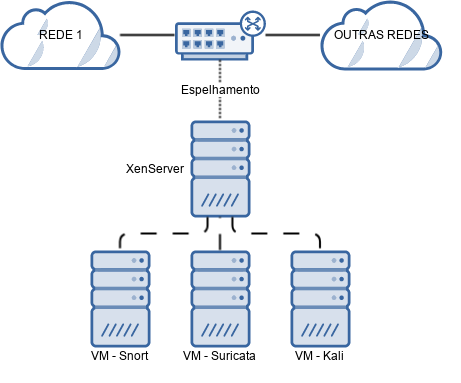
\includegraphics[scale=.65]{infra.png}
\label{fig:infra-ambiente}
\legend{Fonte: Autoria própria}
\end{figure}

Para coleta das informações de uso de recurso de hardware como memória, processamento e I/O das máquinas com os IDSs foi utilizado o \textit{daemon} Collectd \cite{collectd}. Outra opção para esse finalidade é a utilização de um servidor de monitoramento como o Zabbix \cite{zabbix}. A ideia de ter duas ferramentas para essa analise é fazer um comparativo e validar as informações coletadas.

O formato usado para facilitar a análise do \textit{logs} foi JavaScript Object Notation (JSON), um formato simples, leve e de fácil leitura. O Motor de Saída do Suricata já tem suporte a esse tipo de formato o que não acontece no Snort. Para tal, usou-se o IDSTools \cite{py-idstools}, uma coleção de bibliotecas na linguagem python que trabalha para auxiliar o IDS Snort. Dentre os utilitários presentes nessa coleção, temos o idstools-u2json, que converte, de forma continua, arquivo no formato unified2, uma das saídas disponível no Snort, para o formato JSON.

Para analisar os \textit{logs}, usou-se uma infraestrutura que combina três ferramentas:

\begin{alineas}
\item \textbf{Kibana} \cite{kibana}: Uma plataforma de análise e visualização desenhada para trabalhar com os índices do Elasticsearch \cite{elasticsearch}, a grosso modo, podemos dizer que ela é uma interface gráfica para o Elasticsearch. 
\item \textbf{Elasticsearch}: Um motor de busca e análise altamente escalável, capaz de armazenar, buscar e analisar uma grande quantidade de dados em tempo próximo ao real. 
\item \textbf{Logstach} \cite{logstach}: Um motor de coleta de dados em tempo real, unificando os dados de diferentes fontes dinamicamente, normalizando-os nos destinos escolhidos.
\end{alineas}

Dessa forma centralizou-se os \textit{logs}, facilitando a visualização e analise das ocorrências dos IDSs. 

\section{Testes Realizados} \label{sec:testes}
%Quais os testes realizados com justificativa ?
%Descrição dos testes. Quais os testes foram realizados ?
Os testes realizados são simulações de passos que uma pessoa má-intencionada iria tomar para alguma tentativa de invasão, entende-se por invasão, qualquer tipo de violação e alteração não autorizada de um serviço ou \textit{host}.

O passo inicial seria um estudo do alvo utilizando várias técnicas mas principalmente a engenharia social, analisando as pessoas que trabalharam na organização, enviando spam e \textit{phishing} na tentativa de capturar dados como senhas de acesso. 

Posteriormente, o atacante iria observar o tráfego da rede, verificando os serviços que o alvo oferece, a procura de alguma senha desprotegida (não criptografada). Esse passo inicial não será aplicados nos testes pois seria impossível o IDS detectar.

O passo seguinte seria uma garimpagem de informações e mapeamento da rede, a procura de um \textit{host} vulnerável. A ferramenta escolhida para essa finalidade é o Nmap \autoref{sec:nmap}. 

No primeiro teste de \textit{scan}, usou-se o parâmetro '-F', habilitando a modo \textit{fast} do Nmap. Nesse modo, são verificadas apenas a portas especificadas no arquivo nmap-services, na instalação padrão esse arquivo vem com 27372 portas descritas. Isso é muito mais rápido que verificar todas as 65535 portas tcp e 65535 portas udp, possíveis em um \textit{host}.

\begin{lstlisting}[language=bash, frame=single]
    nmap -F 192.168.1.107
\end{lstlisting}

O segundo teste, usou-se o parâmetro '-sV' do NMAP. Essa opção habilita a descoberta de versões, tentando determinar os protocolos de serviços, o nome da aplicação, o número da versão, o nome do \textit{host} (utilizando o DNS reverso), tipo de dispositivo, sistema operacional usado, entre outras informações. Essas informações são de grande valor pois, a partir delas, pode-se explorar vulnerabilidades conhecidas de uma determinada versão de um serviço \cite{nmap}.

\begin{lstlisting}[language=bash, frame=single]  
    nmap -sV 192.168.1.107
\end{lstlisting}

De posse de um alvo em potencial, próximo passo seria rodar um \textit{scanner} de vulnerabilidade, em busca de brejas já conhecidas, e que, geralmente por descuido do administrador, não foi fechada. Essas brejas podem ter várias origem, desde uma versão do serviço com \textit{bugs} ou uma má configuração. Para esse teste, usou-se o OpenVAS (\autoref{sec:openvas}).

Alguns configurações são necessárias nessa etapa. Primeiramente, deve-se definir o alvo, tal configuração é feita através do caminho "\textit{Configuration > New target}", a \autoref{fig:openvas-newtarget} mostra a janela aberta, nela temos que definir um nome para o alvo e o IP ou a faixa de IP's, as outras configurações serão deixadas com o padrão.

\begin{figure}[!htb]
\centering
\caption{Definição do alvo no OpenVAS}
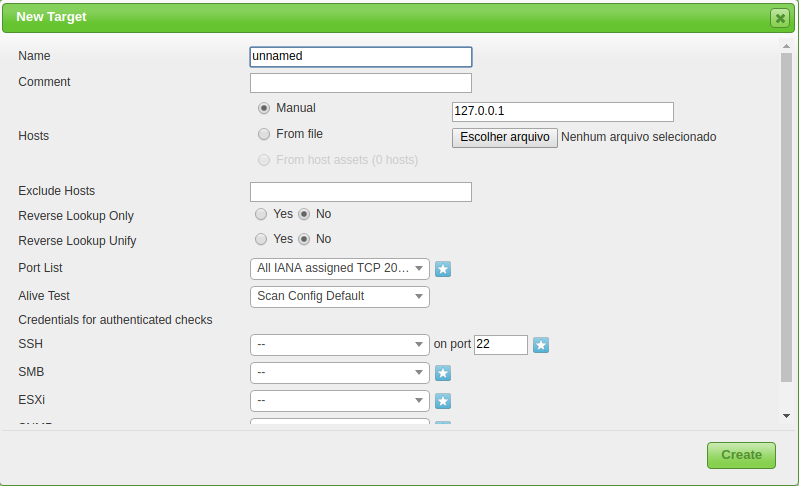
\includegraphics[scale=.55]{openvas-newtarget.png}
\label{fig:openvas-newtarget}
\legend{Fonte: Autoria própria}
\end{figure}

A realização do scan é feita através do caminho "\textit{Scans > Tasks > New Task}", na \autoref{fig:openvas-newtask} mostra a janela aberta, nela precisamos definir no nome da \textit{task} e o alvo, que foi definido anteriormente, as outras opções serão deixadas com o padrão. 

Por padrão, quando uma \textit{task} é criada, o \textit{scan} é automaticamente executado. Esse processo pode demorar, isso depende de quantos alvos foram definidos. Ao final, um relatório é exibido com as vulnerabilidades encontradas e categorizadas (\textit{high, medium, low}) de acordo com a sua severidade. Além disso, o OpenVAS exibe um sumário, descrevendo a(s) falha(s) encontrada(s) e como resolver ou mitigar o problema.

\begin{figure}[!htb]
\centering
\caption{Configuração de um \textit{task} de scan no OpenVAS}
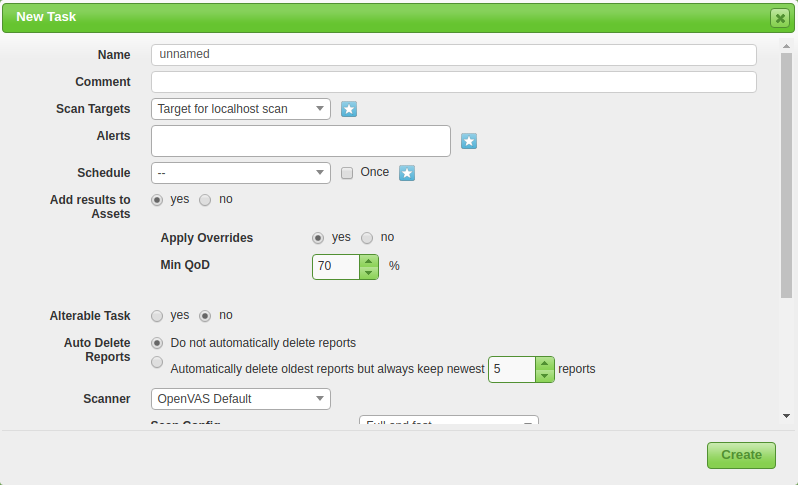
\includegraphics[scale=.55]{openvas-newtask.png}
\label{fig:openvas-newtask}
\legend{Fonte: Autoria própria}
\end{figure}

Outro teste realizado determinará a capacidade das ferramentas de detectar ataques de negação de serviço (\autoref{sec:negação}). Existem várias técnicas para realizar esse tipo de ataque, o usado nesse trabalho foi o TCP SYN FLOOD. 

Quando um cliente tenta começar um conexão TCP com um servidor, são trocados, entre eles, uma série de mensagens (\textit{Three-Way Handshaker}). O TCP SYN FLOOD consiste em enviar uma sequência de requisições SYN para o alvo, sobrecarregando-o diretamente na camada de transporte e indiretamente na camada de aplicação.

Para tal, usou-se o Metasploit Framework (\autoref{sec:metasploit}). Primeiramente, entrou-se no console de linha de comando, para acessar, basta, no terminal, digitar \textit{msfconsole}. Existe um modulo no Metasploit chamado \textit{synflood}, para utilizar esse modulo, é necessário definir o IP do alvo e o IP de onde partirá o ataque. Abaixo segue os comandos usados no \textit{msfconsole}.

\begin{lstlisting}[language=bash, frame=single]
use auxiliary/dos/tcp/synflood

msf auxiliary(synflood) > set rhost 192.168.1.107 (target IP)

msf auxiliary(synflood) > set shost 192.168.1.105 (attack IP)

msf auxiliary(synflood) > exploit
\end{lstlisting}

No ultimo teste, utilizou-se o \textit{framework} Pytbull (\autoref{sec:pytbull}). O Pytbull foi desenvolvido especificamente para realizar testes e validar configurações em IDPS. Na documentação oficial exemplifica algumas arquiteturas que podem ser usadas, 

\section{Resultados} \label{sec:resultados}
%Resultados esperados e obtidos
%Quais os resultados dos testes ??
%Comparação das ferramentas
%Problemas encontrados
\section{Conclusão} \label{sec:conclusão}
%\section{Métricas de Comparação}
%Consumo dos Recursos de Hardware (Memória, Processamento)
%Taxa de Detecção
%Número de Falsos Positivos/Negativos
